%%%%%%%%%%%%%%%%%%%%%%%%%%%%%%%%%%%%%%%%%%%%%%%%%%%%%%%%%%%%%%%%%%%%%%%
%% Einleitung
\section{Einleitung}
\label{sec:einleitung}

Der demographische Wandel stellt die Gesellschaft und die Politik vor ein großes Problem. Nicht nur der fehlende Nachwuchs, der ein Arbeitnehmermangel hinterlässt, sondern auch eine immer älter werdende Gesellschaft stellen Schwierigkeiten dar. Neben kommunalen Problemen, wie teure Infrastruktur, ist die Altersarmut eins der größten Anliegen. Ein sinkendes Rentenniveau und steigende Kosten werden es in Zukunft unmöglich machen für eine gute Pflegeversorgung zu bezahlen  \citep{brunozandonella2013}. Neben den hohen Kosten in der Pflege gibt es auch weitere Faktoren, die zu einer nicht akzeptablen Situation führen. So ist der Pflegeberuf zu unattraktiv für viele junge Menschen, wodurch auch hier ein großes Loch an Arbeitnehmern wahrzunehmen ist. Außerdem führt körperlich anstrengende Arbeit, die in kurzer Zeit ausgeführt werden muss, zu vielen physischen und psychischen Erkrankungen der Pfleger \citep{AOK2004}.

Eine mögliche Lösung liegt in der Technik. Einfach zu bedienende Systeme können den Alltag vereinfachen und so auch älteren Menschen ein selbstständiges Leben ermöglichen. Alltägliche Aufgaben müssten nicht mehr von Pflegekräften übernommen werden, sondern könnten durch Maschinen erledigt werden. Schon heute können einzelne Kleinsysteme Haustätigkeiten, wie Staubsaugen und Rasenmähen, übernehmen. Ein Vorreiter auf diesem Gebiet ist das Roboterland Japan. Dort überlegte sich Kobayashi Hisato, Professor für Maschinenbau und Robotik an der Hosei-Universität in Tokio, schon 1999 Konzepte für Senioren-Service-Roboter \citep{wagner2009tele}. Nach seinen Vorstellungen sollten dabei Roboter nicht autonom arbeiten, sondern von Familienangehörigen ferngesteuert und überwacht werden \citep{kobayashihisato1999}. Neben diesen Konzepten kann man aber auch schon angewandte Robotik in Japans Seniorenpolitik finden. Zwei Musterbeispiele zeigen dabei die unterschiedlichen Anwendungsszenarien für Roboter im privaten Umfeld. \textit{Sinére K\={o}rien} der Firma Matsushita ist ein digitales Seniorenheim. Neben einer Smarthouse Anbindung gehört auch der Roboterteddy K\={o}-chan zur Ausstattung der einzelnen Zimmer (siehe Abbildung \ref{fig:roboTeddy}). Dieser dient als Unterhaltungsroboter und Kommunikationsgerät mit den Pflegerkräften. So kann mit den Kameraaugen im Teddy eine Aufnahme vom Raum gemacht werden und im Notfall den Pflegekräften eine Alarmmeldung geschickt werden. Weitere Sensoren, zum  Beispiel Gewichtssensoren unter den Betten, geben Informationen über die Abwesenheiten von Patienten \citep{wagner2009tele}. Ein weiterer Anwendungsbereich für Roboter ist die \textit{robotto serap\={\i}} (Robotertherapie). Dabei beschäftigen sich Senioren mit tierähnlichen Robotern, wie Hunden, Seerobben oder Katzen (siehe Abbildung \ref{fig:roboTeddy2}). Im Zentrum der Therapie steht die Interaktion zwischen Patient und Roboter. Die Robotertherapie soll die Patienten aktivieren und deren Tagesabläufe abwechslungsreich gestalten. Außerdem steigert es die Kommunikation zwischen zwei Patienten, die am selben Roboter arbeiten \citep{wagner2009tele}. 

 \begin{figure}
 	\centering
 	\subfigure[Roboterteddy K\={o}-chan. Bildquelle: \citep{panasonic2005}]{%
 		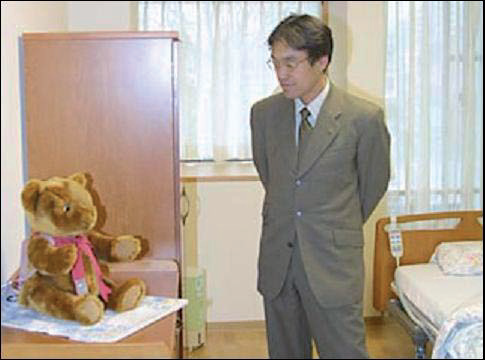
\includegraphics[scale=0.6]{fig/roboteddy}
 		\label{fig:roboTeddy}}
 	\hfill
 	\subfigure[Roboterkatze zur Therapie. Bildquelle: \citep{wagner2009tele}]{%
 		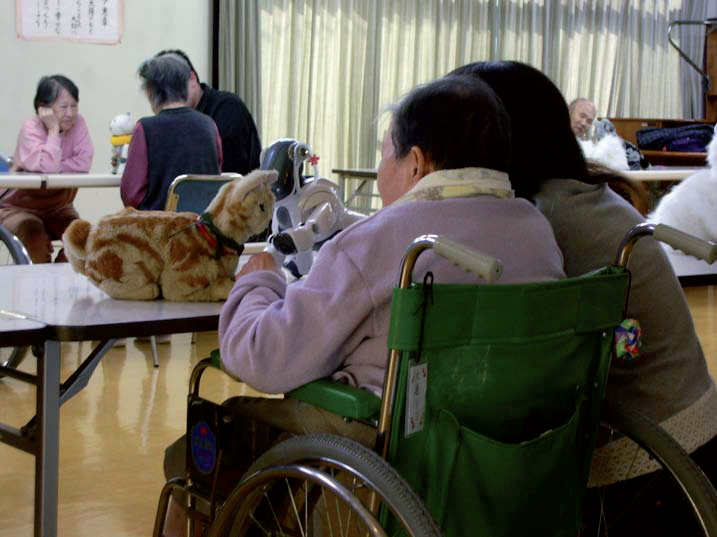
\includegraphics[scale=0.4]{fig/robocat}
 		\label{fig:roboTeddy2}}
 	\caption{Roboter in Seniorenheimen}
 	\label{fig:robSenioren}
 \end{figure}

Nicht nur in Japan, sondern auch in Deutschland wird sich mit dem Thema \textit{Care(rob)bots} befasst. So finden sich unter dem Stichpunkt \textit{Mensch-Maschine-Entgrenzungen} Studien zu der Thematik. Andere Untersuchungen befassen sich mit der Gegenseite, der Akzeptanz der Senioren für Roboter. So ergab eine Befragung der VDE-Studie "Mein Freund der Roboter", dass eine Mehrheit (56\%) der Senioren Robotern im Haushalt offen gegenüber stehen und diese einem Pflege-/Altersheim vorziehen würden. Neben den bekannten Staubsauger- und Rasenmährobotern, sind es auch zukünftige Anwendung, wie ein roboterisierter Rollstuhl, die hohe Akzeptanzwerte erreichen. Die Studie zeigte aber auch, dass Senioren zunächst Robotern skeptisch gegenüberstehen. Spontan lehnten 40 Prozent der Senioren Roboter in ihrem privaten Umfeld ab, 60 Prozent empfanden Robotik sogar als unheimlich. Jedoch zeigte sich, dass der Wunsch nach einer selbstständigen Lebensführung ein starker Faktor für die Akzeptanz ist. Dadurch ergibt sich eine Beliebtheit für Serviceroboter. So sind Roboter sehr beliebt, die abgrenzbare Tätigkeiten im Haushalt selbständig erledigen. Wichtige Kriterien für die Akzeptanz waren zudem die intuitive Bedienbarkeit, die Robustheit und die Flexibilität gegenüber unterschiedlicher Handicaps. Auch menschliche Faktoren wie Geduld, Verständnis, Höflichkeit und Achtung der Intimsphäre waren den Anwendern wichtig \citep{dr.sibyllemeyer2011}.

Neben den sozialen Forschungen gibt es in Deutschland auch ingenieurwissenschaftliche Ergebnisse auf diesem Gebiet. So beschäftigt sich das Cluster of Excellence Cognitive Interaction Technology (CITEC) in Bielefeld, zusammen mit der Stiftung Bethel, in der Forschung auf dem Gebiet der Unterstützung für Demenzkranke. Die dort entwickelten Assistenzsysteme helfen den Patienten unter anderem beim Zähneputzen und geben ihnen so ein Stück Selbstständigkeit zurück \citep{peters2010task}. 

Viele Forschungen und Entwicklungen beschäftigen sich momentan mit der Mensch-Maschine/ -Roboter Beziehung. Dabei geraten die Roboter-Roboter-Interaktionen in den Hintergrund. Heutige Roboter sind keine Allround-Lösungen, sondern meist hochgradig spezialisiert und nur eine Tätigkeit ausführen können (zum Beispiel Saugroboter, Fensterwischroboter und weitere). Deshalb ist die Konfiguration und Koordinierung der Roboter wichtig. Das Szenario in Abbildung \ref{fig:szen1} zeigt, wie solch ein Multi-Robot System aussehen könnte.

\begin{figure}
	\centering
	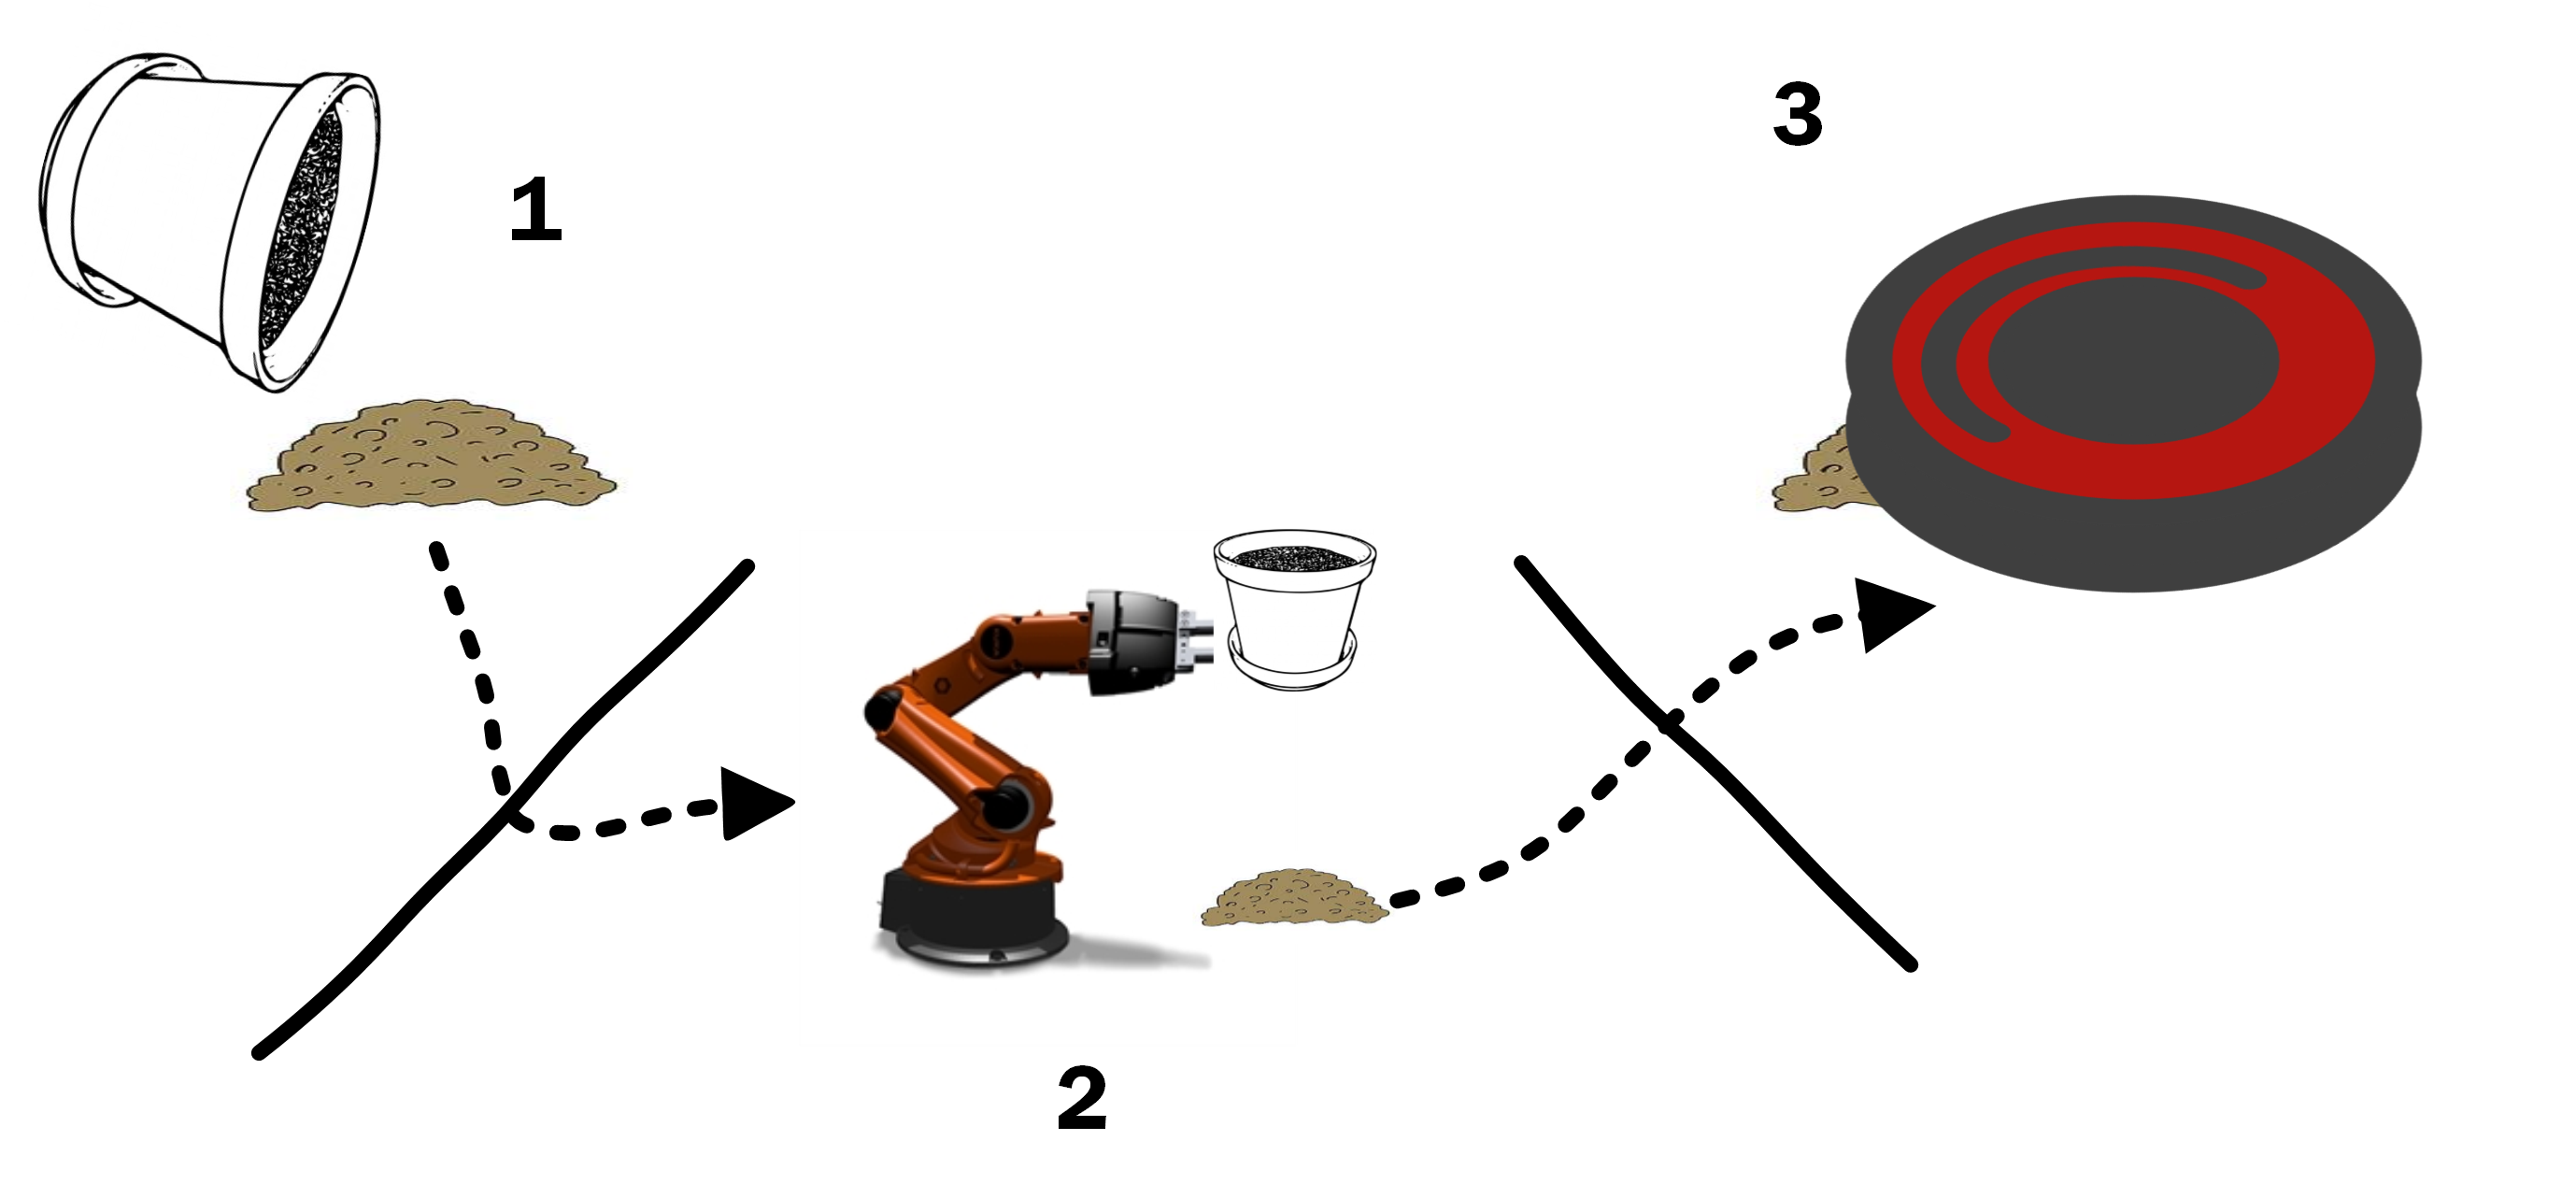
\includegraphics[width=\textwidth]{fig/szen1}   
	\caption[Beispiel Szenario 1]{Mensch A stößt einen Blumentopf um (1). Ein Kamerasystem detektiert, dass der Topf umgefallen ist und Erde auf dem Boden liegt. Ein Roboter mit Arm wird gerufen, der zunächst die Vase aufhebt und an ihren Platz zurückstellt (2). Anschließend wird ein Saugroboter aktiviert, der die Erde wegsaugt (3). Bei schwereren Verschmutzungen wird noch ein Wischroboter bestellt.}
	\label{fig:szen1}
\end{figure}

Dabei führt jeder Agent selbstständig  und unabhängig von den anderen seine Arbeit aus. Die Koordinierung geht immer von der zentralen Steuereinheit aus. Zwischen den einzelnen Robotern findet kein Informationsaustausch statt. Die Agenten arbeiten seriell ihre Aufgaben ab. Die Änderung an dem Szenario in Abbildung \ref{fig:szen2} ändert jedoch die Art der Koordinierung. Dadurch wird ein Informationsaustausch zwischen den einzelnen Robotersystemen nötig. Auch paralleles Arbeiten der Roboter ist dadurch möglich.

\begin{figure}
	\centering
	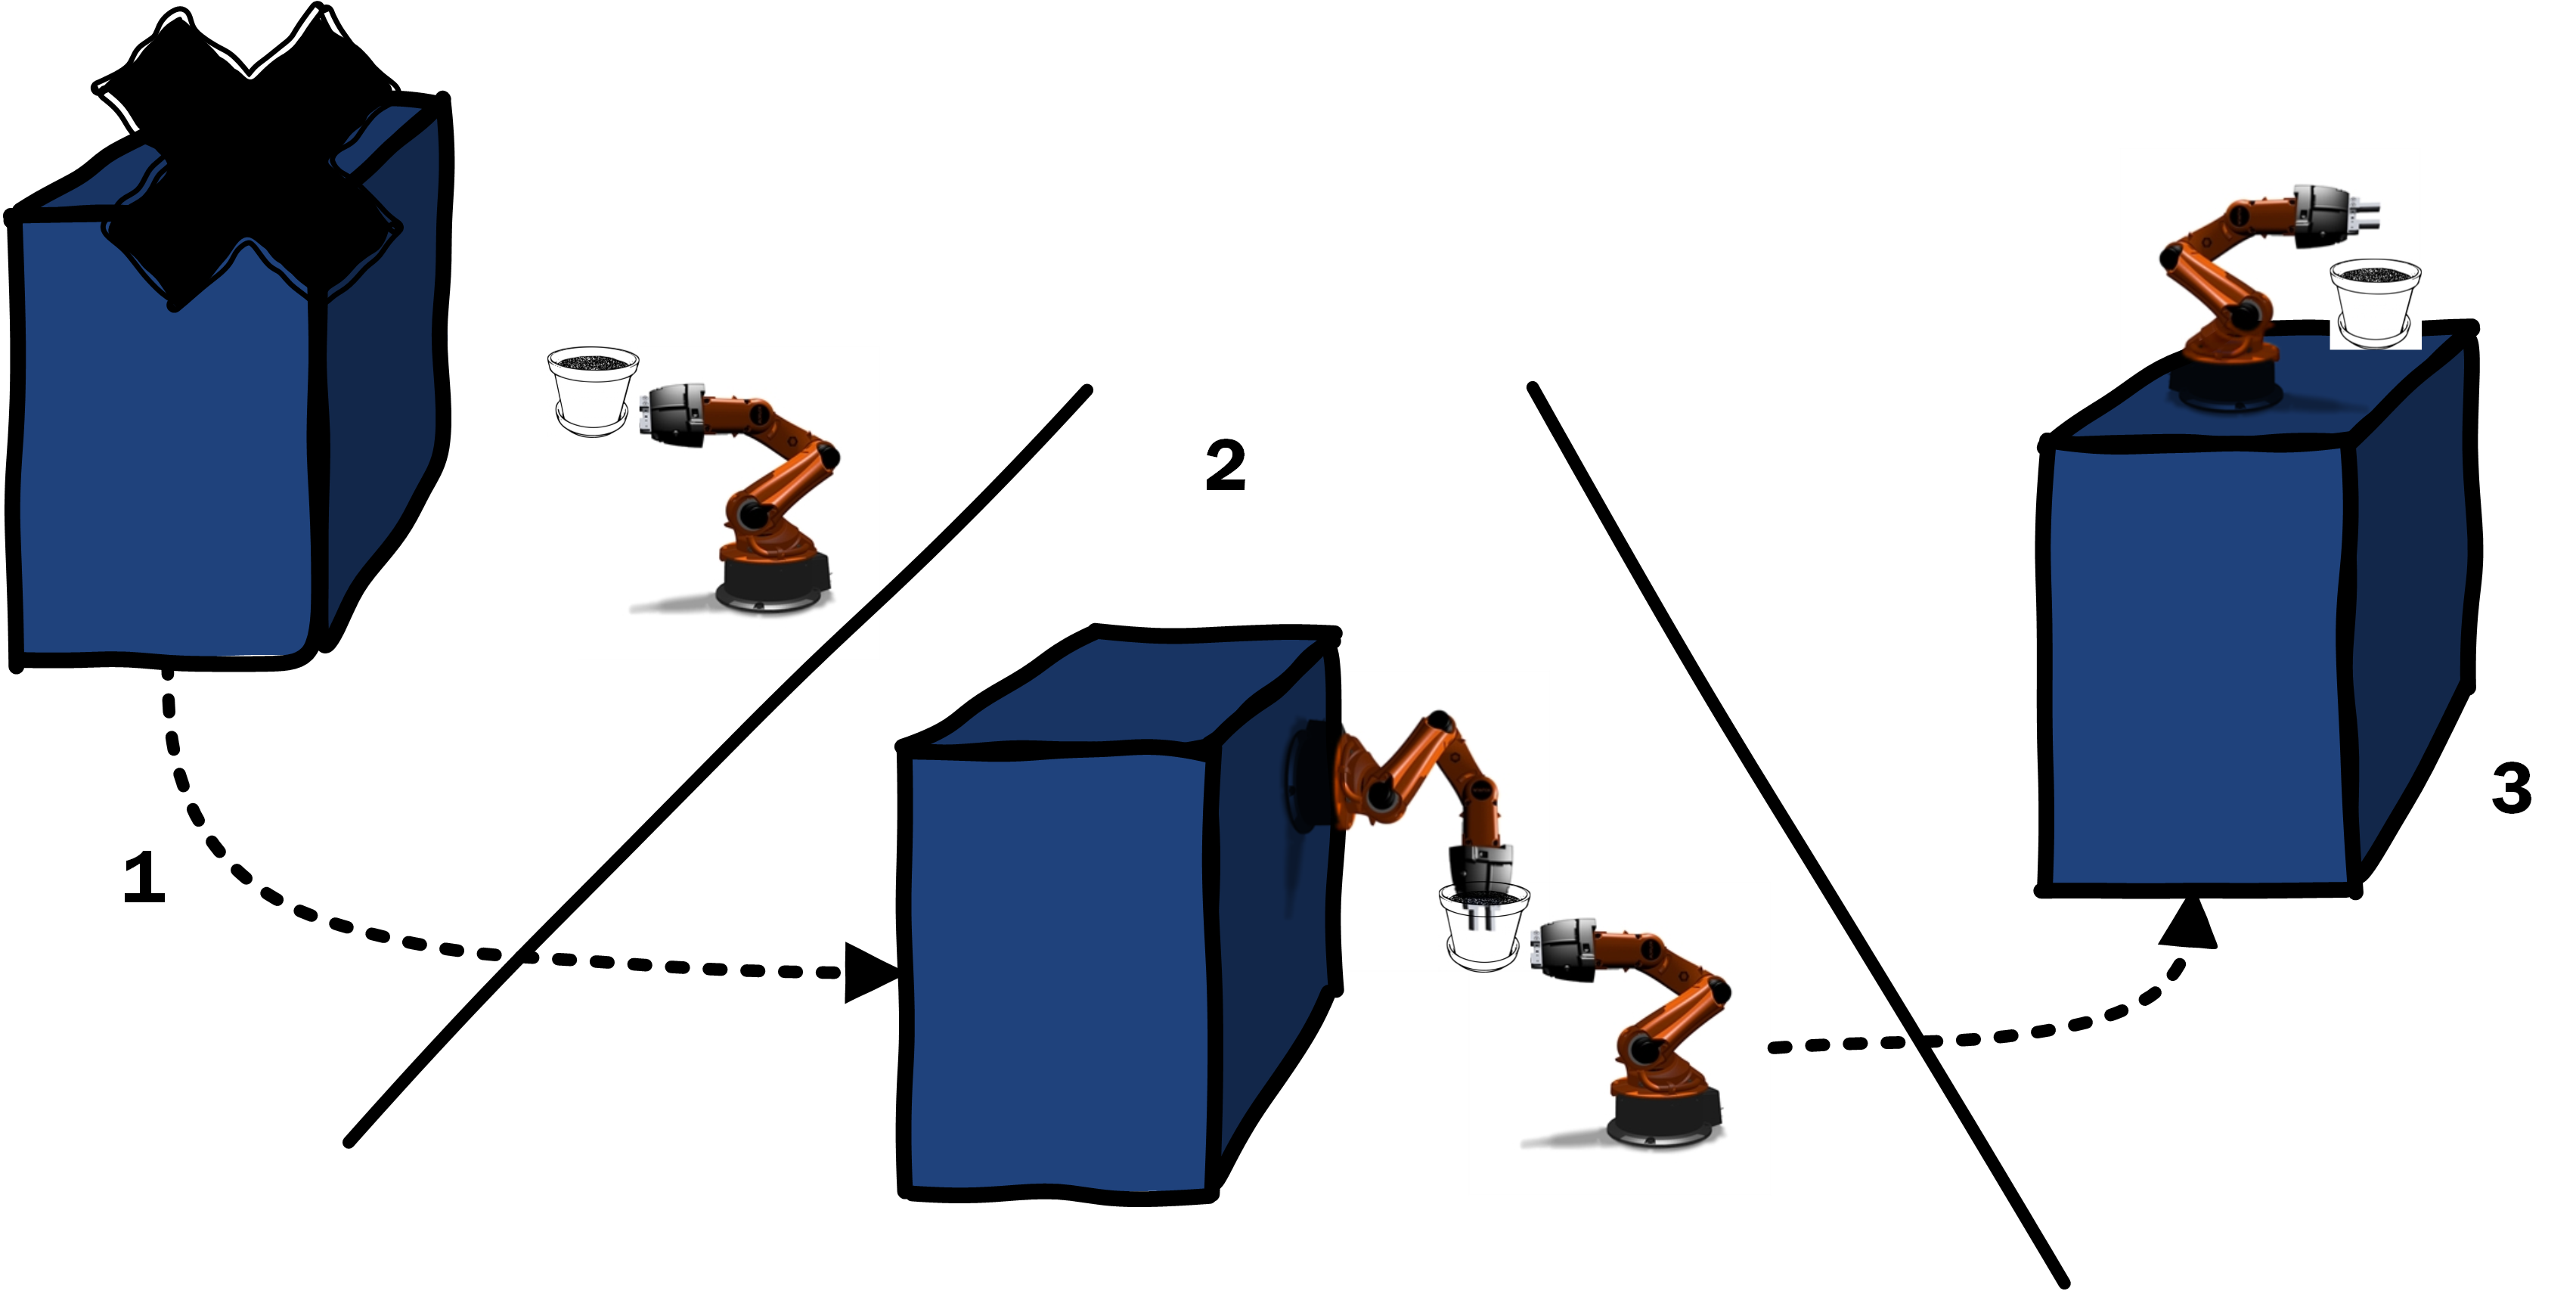
\includegraphics[width=\textwidth]{fig/szen2}   
	\caption[Erweiterung Szenario 1]{Beim Zurückstellen der Vase stellt der Roboter fest, dass er die gewünschte Position nicht erreichen kann(1), weil sein Arm zu kurz ist. Da auf der Anrichte noch ein weiterer Arm steht, nimmt er die Kommunikation mit diesem Agenten auf. Sie kommunizieren einen Übergabepunkt und führen ein Übergabemanöver durch. Arm 2 stellt nun die Vase an die gewünschte Position.
	}
	\label{fig:szen2}
\end{figure}


Der zentrale Aspekt dieser Arbeit befasst sich mit dem Aufbau eines Multi-Robot-Systems, kurz MRS. Das Anwendungsszenario ist eine Abstraktion von Szenario 2. Roboter 1 übergibt ein Objekt an Roboter 2. Dabei werden verschiedene Thematiken der Robotik aufgegriffen, untersucht und erläutert. Kapitel \ref{sec:basics} befasst sich mit den Grundlagen auf denen diese Arbeit aufbaut. Neben der Nomenklatur wird die Middleware \textbf{R}obot \textbf{O}perating \textbf{S}ystem, kurz ROS, erläutert. Dabei wird auf den Aufbau, sowie die Kommunikationsschicht von Robotersystemen eingegangen. Anschließend folgt eine kurze Einführung in die mechanischen Grundlagen. Dabei werden die Begriffe rund um die Kinematik erklärt. 

In Kapitel \ref{sec:relatedwork} folgt eine detaillierte Übersicht der zugehörigen Literatur. Zunächst werden Arbeiten um das Thema MRS untersucht. Zentraler Aspekt dieser Thematik ist die Koordinierung von mehreren Robotersystemen. Drauf aufbauend wird das PEIS-Konzept erläutert. In diesem wird eine Nutzung von externen Sensoren für MRS gezeigt. Abschließend wird ein kurzer Einblick in Arbeiten zum Thema Greifen und Übergeben gegeben.

Das anschließende Kapitel \ref{sec:basic-aufbau} beschreibt den Aufbau des Teststandes, sowie die verwendete Hardware. Dabei wird auf die einzelne Sensoren und Aktoren eingegangen. Außerdem werden verschiedene Tests mit Prototypen durchgeführt, um die Genauigkeit und Qualität der Ergebnisse einzuschätzen.

Im Kapitel \ref{sec:entwicklung} werden die zentralen Aspekte dieser Arbeit beschrieben. Nach einer Auflistung von Nicht-Funktionalen Anforderungen, die bei der Entwicklung des MRS berücksichtigt werden sollen, werden einzelne Funktionalitäten des MRS entwickelt. Dabei werden Konzepte und Methoden vorgestellt. Anschließend folgt die Vorstellung der einzelnen Agenten, die für das Szenario benötigt werden. Diesen werden die Funktionalitäten und die Hardware zugewiesen. Diese Agenten werden durch das RATS miteinander verbunden. Diese Architektur bildet eine Schlüsselkomponente dieser Arbeit ab. Aufgabe von RATS ist die Zuweisung und Koordinierung von Aufgaben für unabhängigen Agenten. Diese Agenten können Sensoren, Aktoren oder Roboter sein. Anschließend wird die Entwicklung und Umsetzung einer geometrischen inversen Kinematik beschrieben. Diese ist für eine präzise Steuerung des Arms wichtig. Folgend wird in Kapitel \ref{sec:impl} die Umsetzung der Konzepte aus dem vorherigen Kapitel erläutert. Dazu werden die Algorithmen für verschiedene Funktionalitäten kurz dargestellt. Dabei werden Verfahren der Computer Vision und der Robotik angewandt. 

Zum Ende der Arbeit wird zunächst das entwickelte System in Kapitel \ref{sec:test} getestet und die Ergebnisse bewertet. Dabei wird sowohl auf funktionale, wie auch nicht-funktionale Anforderungen, eingegangen. Außerdem werden Problemstellen gesucht und analysiert, damit in Kapitel \ref{sec:end} im Ausblick Verbesserungsmaßnahmen vorgestellt werden können. Zuvor erfolgt jedoch eine Zusammenfassung der Arbeit. In dieser wird auf die Ergebnisse der Arbeit zurückgeblickt.



